\chapter{Methodology}
\label{methods:intro}
In this chapter, we will take a closer look at the methodological background of our work, on which the experiments in \autoref{experiments:intro} are based. In particular, we will introduce the Neural Cellular Automata (NCAs) we use and their model architecture and discuss some of the peculiarities of NCAs. To do this, we will first introduce the idea of Cellular Automata (CAs) in \autoref{methods:CA} and then, building on that, in \autoref{methods:NCA} Neural Cellular Automata itself. We will first look at NCAs in general and then present the specific architectures we use. After that, in \autoref{methods:NQM} we will discuss the NCA Quality Metric (NQM) as a measure of the variance between different model outputs, which is the basis of our experiments and the central research topic of this thesis. Finally, in \autoref{methods:Robust}, we describe our approaches to evaluate robustness against artifacts and domain shifts.


%%% --- inputs ---
%%%% --- CA --- %%%%
\section{Cellular Automata}
\label{methods:CA}
Cellular Automata (CA) consist of a discrete set of state machines called "cells," a set of possible states where these cells can be located, a fixed neighborhood of these cells to each other, and an update rule. 

For the update rule of a CA, in particular, \begin{enumerate}
    \item that it is executed in discrete time steps,
    \item that the state of a cell $x_{n,m}$ in the next time step $t+1$ is only determined by the states of the cell itself and its direct neighbors in this time step $t$ and
    \item that all cells execute the same update rule.
\end{enumerate}

The founder of CAs is \autocite{vonNeumann:1951}, who used it to try to model self-replicating artificial systems \autocite{Kari:2005:CA_survey}. CAs are used in many scientific disciplines to model non-linear systems \autocite{Pade:2023:HirarchicalNCA}. CAs themselves form a Turing-completed system, but in contrast to Turing machines, all cells calculate in parallel \autocite{Berto:StanfordSurvey_CA:2022}. For example, a more comprehensive survey on CAs can be found at \autocite{Berto:StanfordSurvey_CA:2022}.

As a simple example for visual data, one can imagine the pixels in an image. Then, for example, each pixel can be defined as a cell, the color or gray values of the pixels as the states, and, using the position of the pixels in the image as the neighborhood, e.g., each 3x3 field forms the neighbors of the middle pixel of this field.

The update rule can then be formulated as a 3x3 kernel. Two such examples are given in \ref{fig:ca_exp}. For (1) and (2), the following simple kernels and zero-padding were used: the initial state is on the far left, and the time steps to the right increase by 1:
\begin{align*}
    (1)\    \begin{bmatrix}
                1 & 0 & 0\\
                0 & 0 & 0\\
                0 & 0 & 0
            \end{bmatrix}
            \ , \qquad
    (2)\    \begin{bmatrix}
                0   & 0.5 & 0\\
                0.5 & 0   & 0\\
                0   & 0   & 0
            \end{bmatrix}\\
\end{align*}


\begin{figure}[h!]
    \centering
    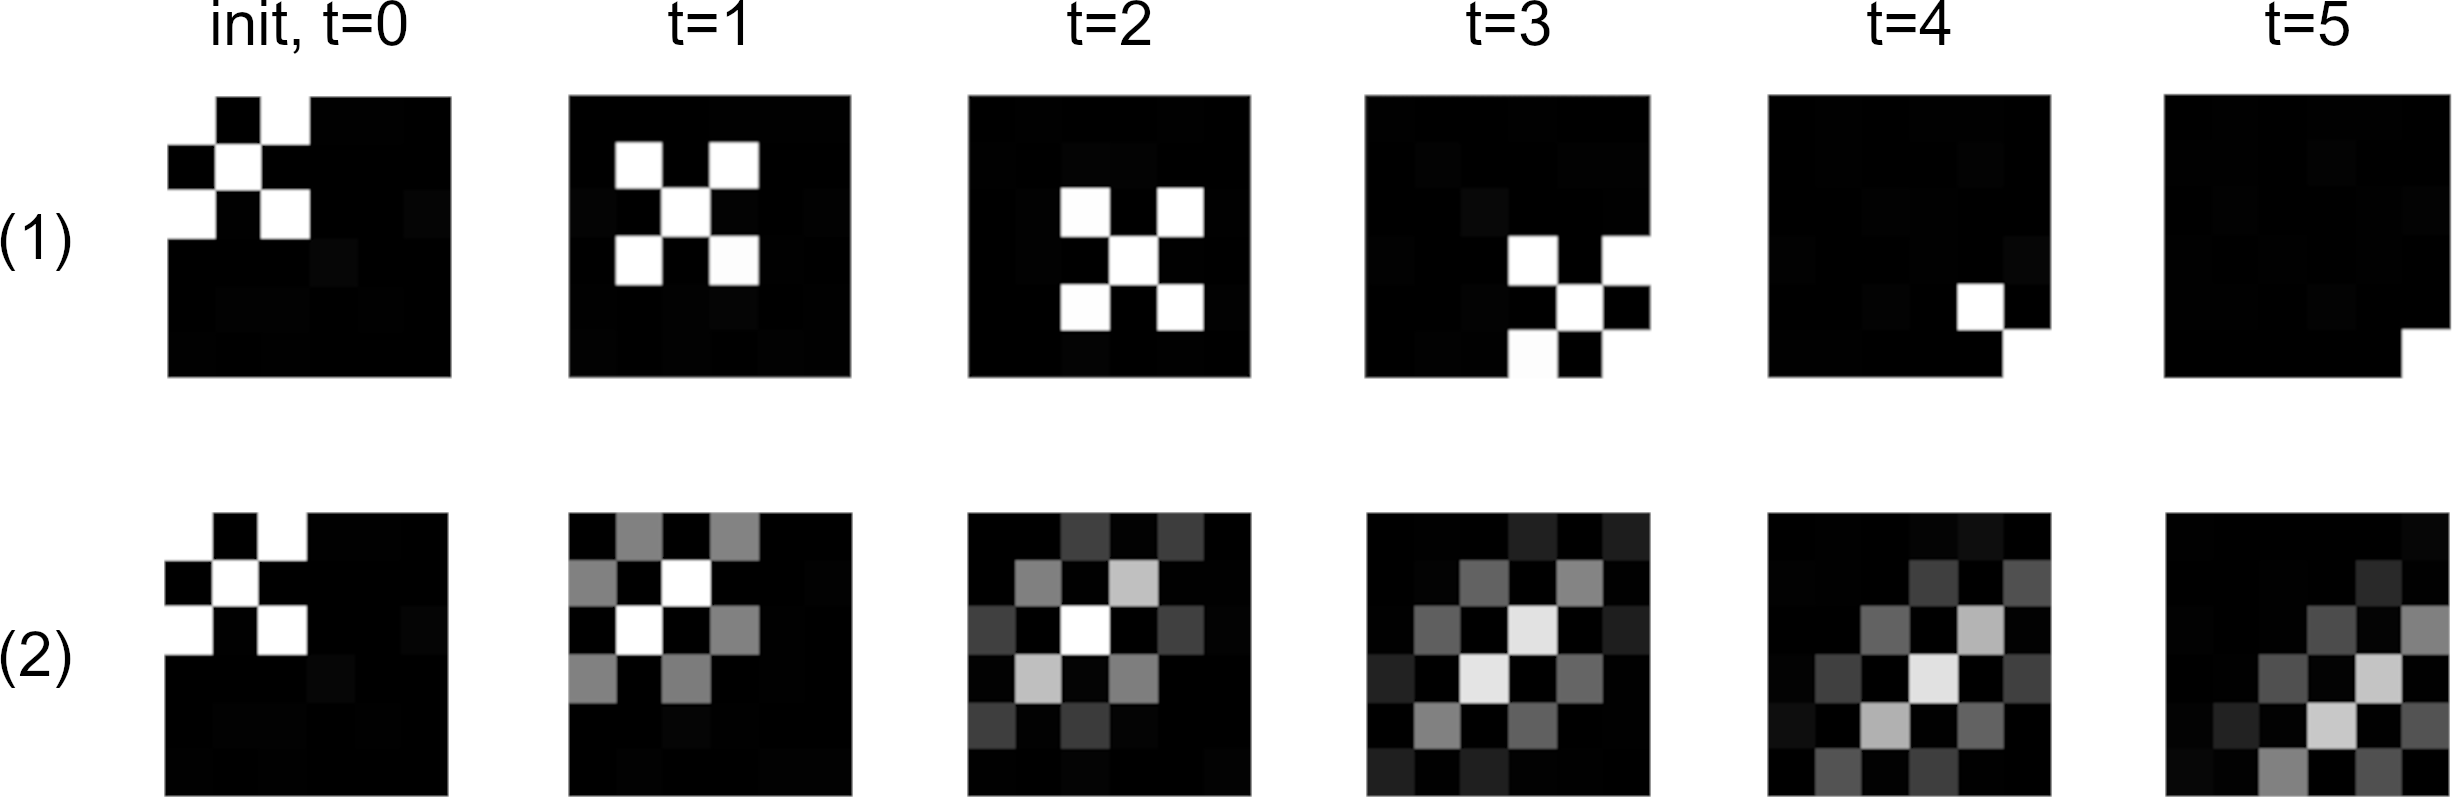
\includegraphics[width=0.9\linewidth]{Graphics/CA_examples.png}
    \caption{Examples of two elementary Cellular Automata on visual data. In a cellular automaton, the state of each cell (e.g., a pixel here) at time step $t+1$ is determined only by the states of the cell itself and its immediate neighbors at time step $t$. In this case, the 3x3 surrounding pixels. The update rules can be described as simple 3x3 kernels. Where time runs from left to right, and the filter is applied to each pixel in each time step. In example (1), there is only a simple shift, and in example (2), the original shape diverges and moves.}
    \label{fig:ca_exp}
\end{figure}

CAs are generally more complex than these simple examples and are not limited to visual data. Instead, among many other things, CAs can be used to simulate and model, e.g., urban evolution, turbulence phenomena, and other fundamental physics, and in general, many discrete dynamical systems, see, e.g., \autocite{Berto:StanfordSurvey_CA:2022}.

Thus, CAs exist for a long time and have a vast application potential. However, the main challenge in directly modeling CAs is often finding a suitable update rule \cite{Gilpin:2019:IntroduceNCA}. In Neural Cellular Automata, these update rules are modeled or trained with a neural network, which is discussed in more detail in the following section.
\section{Neural Cellular Automata}
\label{methods:NCA}
%%%% --- NCA allgemein --- %%%%
Finding an appropriate update rule is often a particular challenge when modeling CAs \cite{Gilpin:2019:IntroduceNCA}. In NCAs, this update rule is learned using a Neural Network (NN). A Neural Cellular Automaton (NCA) is, therefore, a simple (i.e., small) Neural Network. In image processing, the neighborhood of the CA is usually the pixel grid of the input image. Since the update rule is based only on the "direct" neighbors, the NN in an NCA is limited to using only tiny (e.g., 3x3) filter kernels. These architectural choices make the model very small regarding the number of parameters. In addition, unlike other NNs, NCAs do not pass the input through the model just once to generate the output. Instead, the output is fed back into the model for a fixed number of time steps ("inference steps"). In terms of a CA, we let the model update the state (neighborhood) for a fixed number of iterations until we observe the image state. Then, the loss is computed and backpropagated through the model as in any other NN. 

In addition, NCAs also use additional channels, i.e., a hidden state that is many times larger than the input. This hidden state and the input image form the hidden input and output of NCAs, which are used only by the model itself. This allows the model to spread information over the entire image, even if it takes several time steps. The intermediate states are overwritten at each step, i.e., they are not stored, and only a layer the size of the input image is used for the final output. The hidden state is not used for loss calculation.


%%%% --- Models --- %%%%
\label{methods:NCA:Models}
We used two different NCAs for training. The Backbone-NCA and the Med-NCA, as shown in \autoref{fig:NCA_Models}. The Med-NCA is built from two backbone NCAs. Both models are designed for medical image segmentation and were developed by \cite{kalkhof:2023:medNCA}. Although they can be used with different numbers of inference steps and channels, we have consistently used 64 inference steps and 16 channels, which are zero-seeded. Only 15 channels can be used by the model because the first channel is overwritten with the original input image after each inference step. The standard Med-NCA configuration uses 32 channels but provides only 0.01 more performance on Dice, while the 16-channel variant requires 2.5 times fewer parameters. The Backbone NCA is about 0.033 weaker on Dice than the Med NCA, although this also depends significantly on the training set \cite{kalkhof:2023:medNCA}.

Another difference between the NCAs we used and most other NNs is that they use randomness, e.g., during inference. In each inference step of the model, only a random portion of the computed output is returned to the model in the next inference step. That way, the model can continue to compute only a portion of the previous output in the next iteration. The output is randomly masked with $p=0.5$. This is similar to other NCA approaches in image processing \cite{mordvintsev:2020:growingNCA, sandler:2020:imageSegNCA}. The goal behind the randomness is to simulate asynchronous execution. Both models use kernels of size $3\times3$. Overall, tiny but robust models can be trained this way. 


%%%% --- Backbone-NCA --- %%%%
\subsection{Backbone-NCA}
The Backbone-NCA is build with a simple architecture, as can be seen in \autoref{fig:NCA_Models}. The Backbone NCA is only the one on the right. However, it is a powerful segmentation NCA. According to the ablation study by \cite{kalkhof:2023:medNCA}, it is only slightly weaker than the med-NCA on the hippocampus dataset we also used. Because of its simple architecture and good performance, we decided to explore using this NCA and this dataset first and then see if any results could be replicated on the Med-NCA and other datasets.

The backbone NCA consists of 2 conv2d layers, which are limited to a kernel size of $3\times3$ and have an input and output depth corresponding to the channels, i.e., 16 in our experiments. These two layers are arranged in parallel, and their output is merged with the input via two linear layers with intermediate Relu. This model block is run through in each inference step. After each inference step, the generated output is merged with the original input again, forming the input for the next inference step. After all (in our case 64) inference steps, the loss is computed using the ground truth labels and propagated back using the PyTorch \cite{paszke:2019:pytorch} backward function.


%%%% --- Med-NCA --- %%%%
\subsection{Med-NCA}  
\label{methods:NCA:Med-NCA}
The Med-NCA is the more powerful segmentation NCA we use. It is build of two Backbone-NCAs and uses additional up- and downscaling and patching, as can be seen in \autoref{fig:NCA_Models}. For this reason, we decided to test the transferability to another model with this NCA after the results could be achieved with the Backbone NCA. We also used it to test the transferability to the more difficult prostate dataset. 

It is based on 2 Backbone-NCAs connected in series. The first Backbone-NCA works with low-resolution inputs. After the 64 inference steps of the first NCA, the output is scaled up again and sent to the second NCA together with the input image. The second NCA continues to work directly on the output of the first NCA at a higher resolution. The second NCA trains on patches to reduce the VRAM. This is no longer necessary after training. The loss is only calculated on the final output and fed back through both models after the second model has also been executed with 64 inference steps.

\begin{figure}[h!]
    \centering
    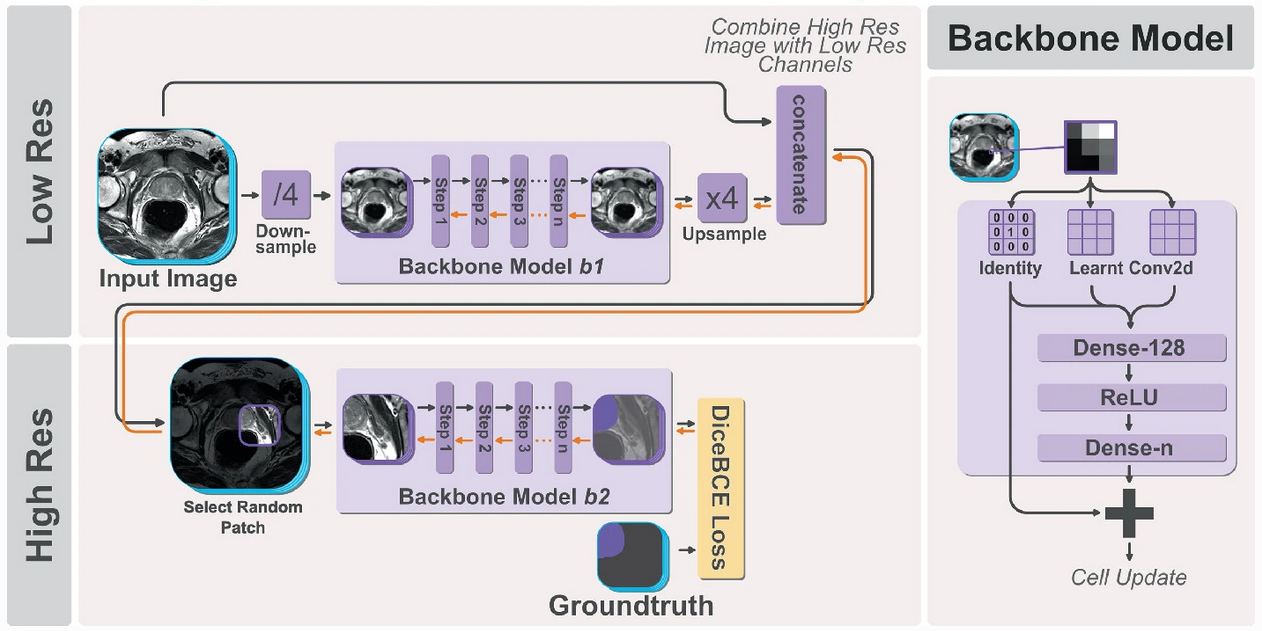
\includegraphics[width=\linewidth]{Graphics/MedNCA_2D.png}
    \caption{The NCAs we used. On the right: The Backbone-NCA, a simple architecture. Whole image: The Med-NCA, using 2 Backbone-NCAs. One training on the whole image, but with low resolution, and one training on high-resolution patches. Patching is not needed after training but reduces VRAM usage. When using the Backbone-NCA alone, we also used the DiceBCE loss. Models and image from \cite{kalkhof:2023:medNCA}.}
    \label{fig:NCA_Models}
\end{figure}

%%%% --- DiceBce Loss --- %%%%
\subsection{DiceBCE Loss}
\label{DiceBCE-Loss}
Both the Backbone-NCA and the Med-NCA use the DiceBCE as the loss. The DiceBCE consists of two parts: the complement of the S{\o}renson-Dice coefficient (Dice or Dice-Loss) and the Binary Cross Entropy (BCE). The DiceBCE is simply the addition of the Dice-Loss and the BCE (\ref{eq:DiceBCE_1}). We use 'Dice' inconsistently for both the complement (i.e. as loss) and the score itself, although it should be apparent from the context what is meant. In particular, only the complement is used as the loss, and only the S{\o}renson-Dice coefficient itself is used as the score for testing, and we never form the complement of the complement or anything like that.

The Dice is the harmonic mean of precision and recall (\ref{eq:DiceBCE_2}), which can be transformed to (\ref{eq:DiceBCE_3}), where TP, FP, and FN stand for True Positive, False Positive, and False Negative, respectively. Overall, the Dice also emphasizes true positives over false positives. For an image volume, where $x_n$ is a prediction $\in(0,1)$ and $y_n$ is a ground truth label $\in(0,1)$ and $n$ is the size of the vectors, i.e., the size of the image volume is $n$. The dice can then be rewritten as (\ref{eq:DiceBCE_4}), where a smoothing factor is added to avoid zero derivatives.

The BCE weights the prediction and rejection ($x_n$ and $(1-x_n)$) logarithmic before multiplying them by the ground truth and then adding them. This element weighting is done for operations on vectors, such as image volumes, where we then reduce by the mean (\ref{eq:DiceBCE_5}). The BCE also maximizes the logarithmic weighted correct predictions of the model and thus minimizes the logarithmic weighted incorrect predictions. The DiceBCE also maximizes the logarithmic weighted correct predictions of the model with a shift towards the true positives.

We used the binary cross entropy function from PyTorch \cite{paszke:2019:pytorch} with reduction for the BCE.
This version of the DiceBCE was used for both the Backbone-NCA and the Med-NCA and proved very effective. Therefore, we used it as a reference in our experiments, and as a starting point for other loss functions we tested.

\begin{align}
    \mathrm{DiceBCE}    &:= 1 - \mathrm{Dice} + \mathrm{BCE},           \label{eq:DiceBCE_1}\\[10pt]
    \mathrm{Dice}       &:= 2 \cdot \frac{\mathrm{precision} \cdot \mathrm{recall}}
                                            {\mathrm{precision} + \mathrm{recall}}          \label{eq:DiceBCE_2}\\[10pt]
                        &= \quad \frac{2 \cdot \mathrm{TP}}
                                   {2 \cdot \mathrm{TP} + \mathrm{FP} + \mathrm{FN}}        \label{eq:DiceBCE_3}\\[10pt]
                        &= \quad \frac{2 \cdot {\sum(x_n \cdot y_n)} +1}
                                   {\sum(x_n) + \sum(y_n) +1}                               \label{eq:DiceBCE_4}\\[10pt]
   \mathrm{BCE}         &:= \mathrm{mean}\ ( -[y_n \cdot \log x_n + (1-y_n) \cdot \log (1-x_n)])        \label{eq:DiceBCE_5}
\end{align}
%%%% NQM %%%%
\section{NCA Quality Metric (NQM)}
\label{methods:NQM}
\begin{figure}
    \centering
    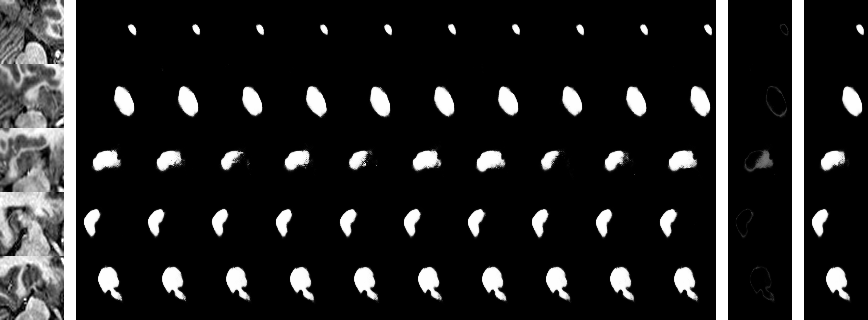
\includegraphics[width=\linewidth]{Graphics/nqm_stack10_epoch_50_var_mu.png}%{Graphics/nca_random_outputs.png}
    \caption{From left to right: Inputs, 10 predictions, Variance, and Mean. As seen here, NCAs produce different outputs on identical inputs each time they are called. Each of the 10 predictions here are outputs of the same model. Therefore, as shown on the right, one can compute a variance and a mean over these predictions. The NQM we introduce here for model optimization reduces this to single values. The outputs are generated from a model in an earlier training state for better visualization.}
    \label{fig:nca_random_outputs}
\end{figure}

%%%% random activation + image example %%%%
As seen in \autoref{methods:NCA}, NCAs are activated randomly to a certain extent. Therefore, they generate different predictions each time they are called, especially with the same input. Examples can be seen in \autoref{fig:nca_random_outputs}. On the far left, one can see five different inputs. Next to them are ten outputs from the same model, shown here for better visualization at an early stage of training. Especially for the middle input, the differences in the outputs can be seen quite well with the naked eye. For the other inputs, the variance over these ten outputs (the second last column on the right) also clearly shows that the model produces different outputs for all input images. Otherwise, the variance should be zero, i.e., completely black. The variance decreases for models with higher epochs but never disappears. It also remains the case that the variance for some inputs is significantly worse than for others.

%%%% Def NQM, from/like John %%%%
\autocite{kalkhof:2023:M3D-NCA} introduced a way to measure this stochasticity of NCAs, caused by random activation, by computing a mean-normalized variance over a stack of such generated outputs and named it the NCA-\textit{Quality-Metric} (NQM). \autocite{kalkhof:2023:M3D-NCA} used this to detect bad segmentation on artificially degenerated data automatically. They defined it as follows, with $v$ as the image volume and $v_i$ as $N=10$ different predictions:

\begin{align}
    \mathrm{NQM} := \frac{\sum_{s\in SD} (s)}  {\sum_{m\in\mu}}, \qquad
    \mathrm{SD} = \sqrt{\frac{\sum^N_{i=1}(v_i-\mu)^2}  {N}}, \qquad
    \mu = \frac{\sum^N_{i=1}v_i}  {N}
\end{align}


This approach has given rise to the question of whether it is possible somehow to pull the NQM inside the training circle, to improve the robustness of the models and not just for the final evaluation. What has been addressed with this thesis. 


%%%% Why to put NQM in the Loss %%%%
The NQM is a single scalar value greater than or equal to zero. With the NQM, a model will perform better if the NQM is smaller. Therefore, the goal of optimizing a model with respect to the NQM can be formalized as a direct minimization problem over the NQM $\min(\text{NQM})$. Other approaches are possible, as discussed in \autoref{conclusions}. Since the object to optimize the NQM can be formalized as a minimization problem, and in the training cycle of a Neural Network, there is already an object to minimize, i.e., the loss, and NCAs are Neural Networks, it is very close to trying to minimize the NQM by using it as the loss function or by including the NQM in the loss function. This is also our approach in this work, and, as we will show, it can lead to a more robust behavior of the model. I.e., it can improve the robustness of the model, as we will see in \autoref{experiments:intro} especially in \autoref{experiments:03.1.0:backbone_hippo:intro}. In \autoref{experiments:03.2.0:med_prost:intro}, \ref{experiments:03.3.0:med_hippo:intro_and_Augmented}, and \ref{experiments:03.4.0:backbone_prost:intro}, we will also see that this is not trivial to transfer to other models and datasets, and that some models may even become less robust.


%%%% Schlussanmerkung  -> evt. nach Conclusions %%%%
The NQM, and therefore this approach, is limited to NCAs and possibly other models with randomness in the output since it is a metric over that randomness. Therefore, the NQM and everything related to it in this paper does not work for most other Neural Networks since the output with these is deterministic.